\chapter{Development}
\label{cha:dev}

Here be some development specifications. We follow the steps for concept A, as highlighted in \cref{cha:back}, \cref{sec:back_A}. In \cref{sec:dev_bck} we discuss the back-end, while \cref{sec:dev_frt} will focus on front-end development.

\section{Back-end}
\label{sec:dev_bck}

Server stuff here. See \cref{eq:my_equation} and \cref{eq:aligned,eq:my_other_equation} that explains the maths behind application.

\begin{equation}~\label{eq:my_equation}
    B = \sum_{\ratioA \in A} \ratioA \times \epsilon
\end{equation}
\myequations{My Equation for B}

\begin{align}
	X & = a^{\epsilon} \nonumber \\
	Z & = \frac{\sqrt{A \times B}}{\sum_{\gamma \in \Gamma} \gamma} \label{eq:aligned}
\end{align}
\myequations{System for X Z}

\begin{equation}~\label{eq:my_other_equation}
    x(r) =
        \begin{dcases*}
		a^2 + \sqrt{3} b & if $r$ is even \\
		a^2 + \frac{\sqrt{3}}{2} b & if $r$ is odd
		\end{dcases*}
\end{equation}
\myequations{Equation for x}

The algorithm for X (\cref{alg:euclid}) has such and such advantages. The Pyhton implementation is shown in \cref{lst:gcd}.

\begin{algorithm}
\caption{Euclidean Algorithm}\label{alg:euclid}\myalgorithms{Euclidean Algorithms}
\begin{algorithmic}[1]
\Function{Euclid}{$a,b$}\Comment{Finding the GCD of $a$ and $b$}
\While{$b \neq 0$}
    \State $t \gets b$
    \State $b \gets a \mod b$
    \State $a \gets t$
\EndWhile
\State \textbf{return} $a$
\EndFunction
\end{algorithmic}
\end{algorithm}

\lstinputlisting[language=Python, caption=Python example of GCD, label={lst:gcd}]{2_main_body/code/gcd.py}

\section{Front-end}
\label{sec:dev_frt}

Interface specs here. See the mockup for interface in \cref{fig:mockup_front-end}\footnote{Complete details in \cref{app:screen}, page \pageref{app:screen}}.

In \cref{fig:flowchart_a} we detail the data flow for process A and while process B is shown in \cref{fig:flowchart_b}.

\begin{figure}[ht]
    \centering
    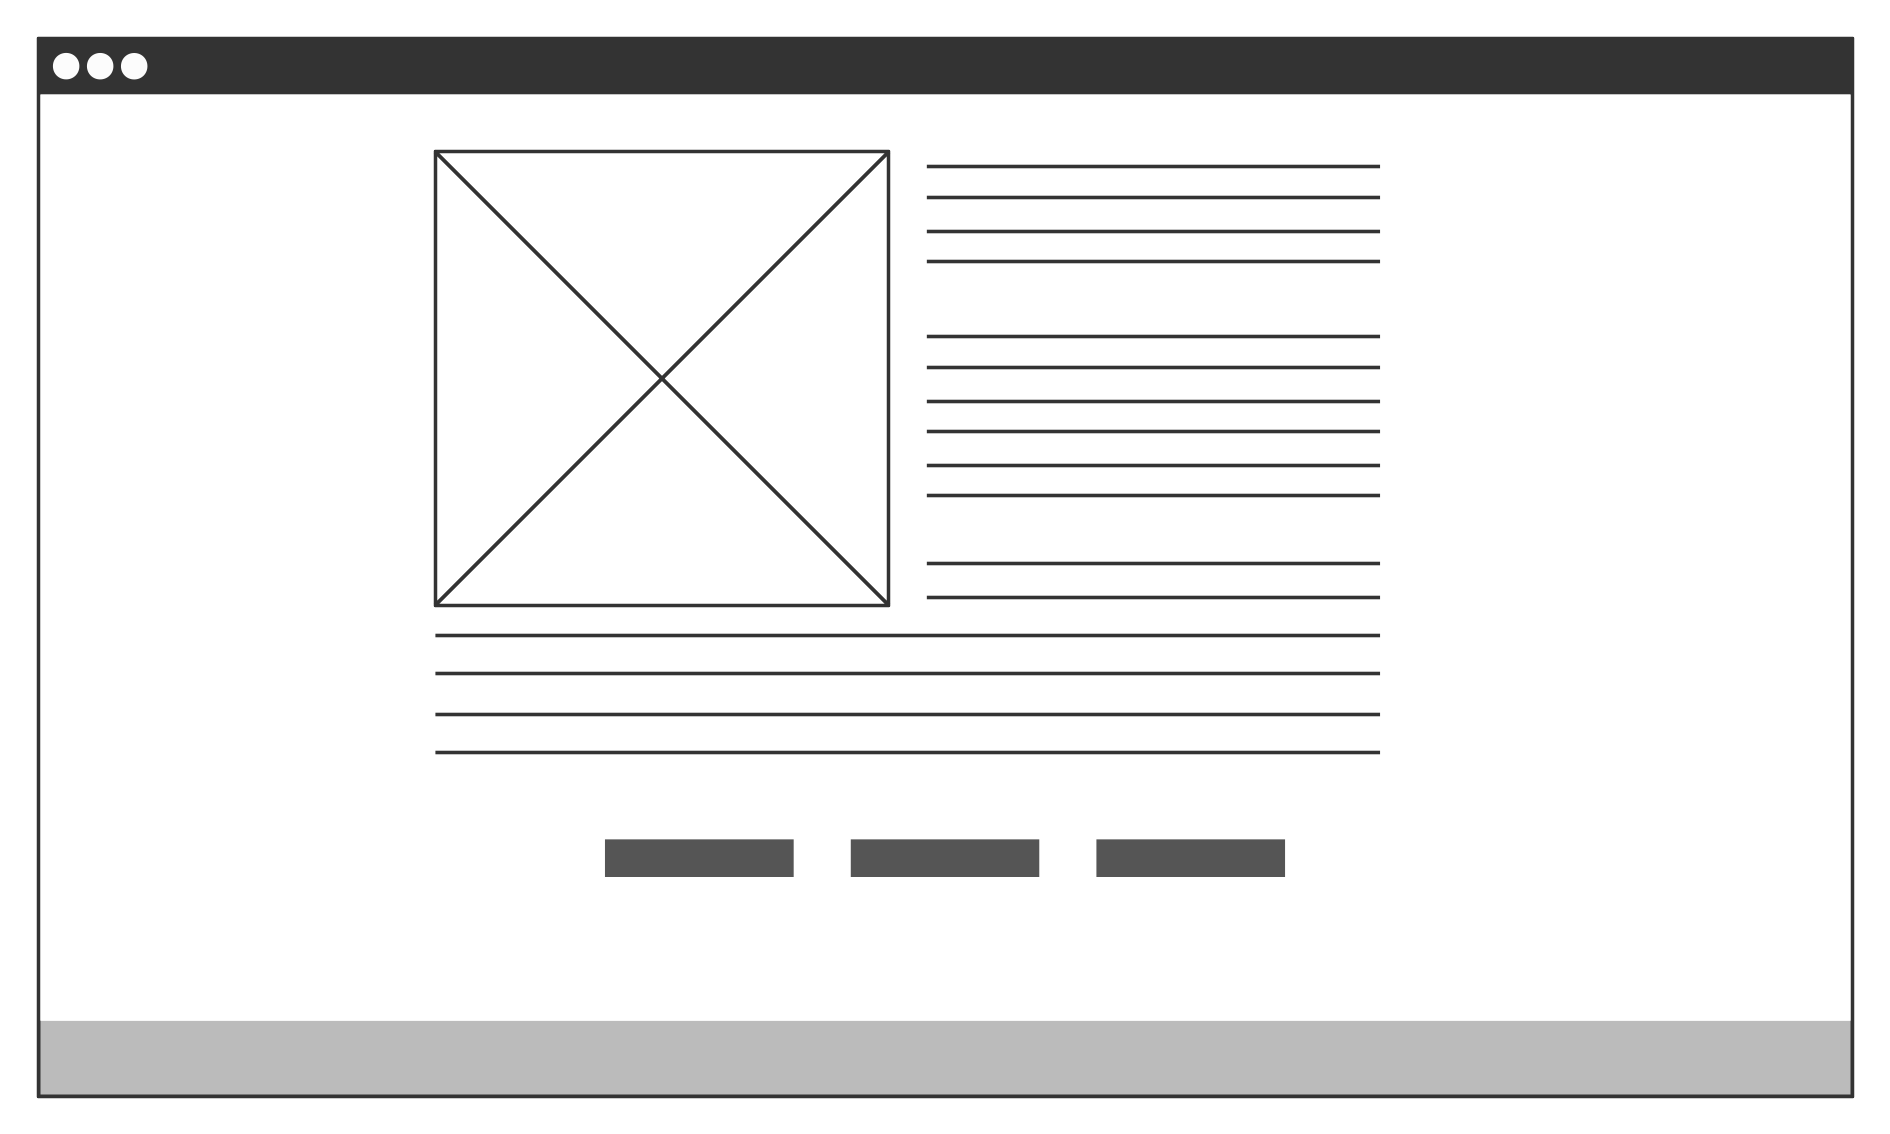
\includegraphics[width=.7\textwidth]{2_main_body/images/mockup.png}
    \caption[Front-end mockup]{Front-end mockup. With an added description to help the reader (won't appear in list of figures).}
    \label{fig:mockup_front-end}
\end{figure}

\begin{figure}[ht]
    \centering
    \hspace{1cm}
    \begin{subfigure}{.35\textwidth}
        \centering
        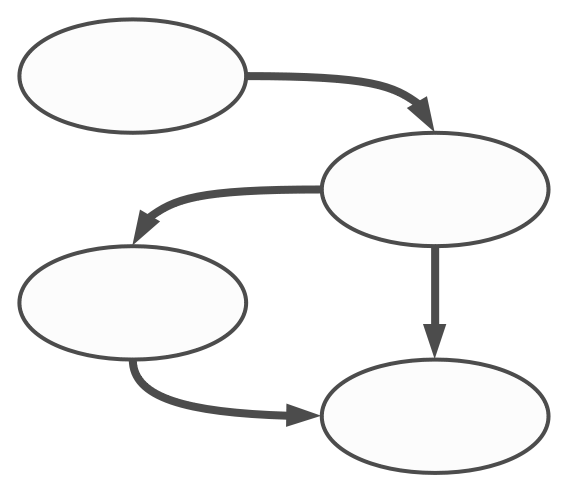
\includegraphics[width=\columnwidth]{2_main_body/images/flowchartA.png}
        \caption{Flowchart A.}~\label{fig:flowchart_a}
    \end{subfigure}
    \hfill
    \begin{subfigure}{.35\textwidth}
      \centering
        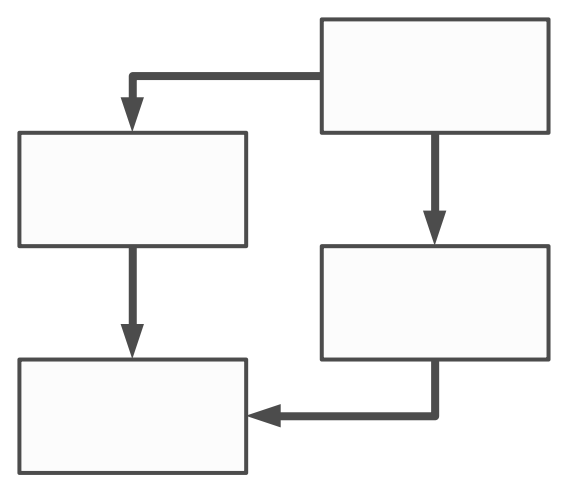
\includegraphics[width=\columnwidth]{2_main_body/images/flowchartB.png}
        \caption{Flowchart B.}~\label{fig:flowchart_b}
    \end{subfigure}
    \hspace{1cm}
    \caption[Flowcharts]{Flowchart for some processes.}~\label{fig:flowcharts}
\end{figure}

\section{Conclusion}
\label{sec:dev_concl}

This chapter has detailed our system implementation. In particular, we have divided the processes into the back-end (\cref{sec:dev_bck}) and the front-end (\cref{sec:dev_frt}).

In the next chapter, \cref{cha:eval}, we evaluate our system.